\documentclass{beamer}
%\documentclass[xcolor=dvipsnames]{beamer}
\usepackage[spanish]{babel}
\usepackage[utf8]{inputenc}
\usepackage{graphicx}

\newcommand{\beamer}{\textsc{beamer}}
\newtheorem{definicion}{Definición}
\newtheorem{ejemplo}{Ejemplo}

%%%%%%%%%%%%%%%%%%%%%%%%%%%%%%%%%%%%%%%%%%%%%%%%%%%%%%%%%%%%%%%%%%%%%%%%%%%%%%%

\title[Presentacion con Beamer]{Series de pontencias de Taylor: ln(x)} %No lo ponemos dentro del begin porque ya están predefinidos
\author[Técnicas experimentales{ULL}]{Yoselin Armas Ramos y Bianca E. Kennedy Giménez}
\institute[ULL]{Universidad de La Laguna}
\date[16-05-14]{16 de Mayo de 2014}
%%%%%%%%%%%%%%%%%%%%%%%%%%%%%%%%%%%%%%%%%%%%%%%%%%%%%%%%%%%%%%%%%%%%%%%%%%%%%%%

\usetheme{Madrid}

%%%%%%%%%%%%%%%%%%%%%%%%%%%%%%%%%%%%%%%%%%%%%%%%%%%%%%%%%%%%%%%%%%%%%%%%%%%%%%%
\definecolor{pantone254}{RGB}{122,59,122}
\definecolor{pantone3015}{RGB}{0,88,147}
\definecolor{pantone432}{RGB}{56,61,66}
\setbeamercolor*{palette primary}{use=structure,fg=white,bg=pantone254}
\setbeamercolor*{palette secondary}{use=structure,fg=white,bg=pantone3015}
\setbeamercolor*{palette tertiary}{use=structure,fg=white,bg=pantone432}
\setbeamercolor*{palette sidebar primary}{use=structure,fg=pantone254}
\setbeamercolor*{palette sidebar tertiary}{use=structure,fg=pantone3015}
\setbeamercolor*{block title}{bg=pantone3015,fg=white}
\setbeamercolor*{alerted text}{fg=pantone432}
\setbeamercolor*{item projected}{fg=pantone254}
\setbeamercolor*{section in toc shaded}{use=structure,fg=structure.fg}
\setbeamercolor*{section in toc}{fg=pantone3015}
\setbeamercolor*{subsection in toc shaded}{fg=pantone3015}
\setbeamercolor*{subsection in toc}{fg=pantone432}

%%%%%%%%%%%%%%%%%%%%%%%%%%%%%%%%%%%%%%%%%%%%%%%%%%%%%%%%%%%%%%%%%%%%%%%%%%%%%%%
\begin{document}
  
%++++++++++++++++++++++++++++++++++++++++++++++++++++++++++++++++++++++++++++++  
\begin{frame}

  \includegraphics[width=0.15\textwidth]{img/ullesc.eps}
  \hspace*{7.5cm}
  \includegraphics[width=0.16\textwidth]{img/fmatesc.eps}
  \titlepage
  \begin{center}
  \begin{scriptsize}
     Facultad de Matemáticas \\
     Universidad de La Laguna
  \end{scriptsize}
  \end{center}

\end{frame}
%++++++++++++++++++++++++++++++++++++++++++++++++++++++++++++++++++++++++++++++  

%++++++++++++++++++++++++++++++++++++++++++++++++++++++++++++++++++++++++++++++  
\begin{frame}
  \frametitle{Índice}  
  \tableofcontents[pausesections]
\end{frame}
%++++++++++++++++++++++++++++++++++++++++++++++++++++++++++++++++++++++++++++++  



\section{Motivación y Objetivos}


%++++++++++++++++++++++++++++++++++++++++++++++++++++++++++++++++++++++++++++++  
\begin{frame}

\frametitle{Motivación}

\begin{definicion}
El objetivo de esta práctica es demostrar los conocimientos adquiridos en Latex, Beamer y Python en el transcurso de la asignatura de Técnicas Experimentales.

\end{definicion}
\begin{center}
\begin{itemize}
\item \LaTeX{} 
\pause
\item Beamer
\pause
\item Python 
\pause
\end{itemize}
\end{center}
\end{frame}
%++++++++++++++++++++++++++++++++++++++++++++++++++++++++++++++++++++++++++++++  

%++++++++++++++++++++++++++++++++++++++++++++++++++++++++++++++++++++++++++++++  
\begin{frame}

\frametitle{Objetivos }


  \begin{itemize}
  \item
   Aplicaremos los programas ya mencionados en la realización de un informe sobre la función logaritmo neperiano y su desarrollo de Taylor.


  \item
   implementaremos un programa en Python que nos ayudará a realizar varios experimentos para respaldar nuestras afirmaciones sobre el tema planteado.

  \end{itemize}

\end{frame}
%++++++++++++++++++++++++++++++++++++++++++++++++++++++++++++++++++++++++++++++  

\section{Fundamentos Teóricos}

\begin{frame}
\frametitle{Fundamentos Teóricos}
\subsection{Historia} %Abrimos una sección

\begin{itemize}
\item El filósofo griego Zenón y sus paradojas.
\item Revolución filosófica.
\item Siglo VXI,Madhava de Sangamagrama y los primeros usos de la serie de Taylor.
\item James Gregory y su interés por las Series de Taylor,series de Maclaurin.
\item En el siglo XVIII ,el matemático británico Brook Taylor presentó de manera formal el Desarrollo de Taylor.
\end{itemize}
\end{frame}


\begin{frame}
\subsection{Series de Taylor}
\frametitle{Series de Taylor.}
\begin{figure}[!th]
\begin{center}

\includegraphics[width=0.20\textwidth]{img/taylor.eps}
\caption{Brook Taylor}
\end{center}
\end{figure}
\begin{itemize}
\item El desarrollo de Taylor parte de una serie infinita y da como resultado un resultado finito.
\item Polinomio de Taylor:
\end{itemize}
 \[ P_{(n,a)} = f(a)+\frac{f'(a)}{1!}(x-a)+\frac{f''(a)}{2!}(x-a)^2+\cdots+\frac{f^{(n)}(a)}{n!} (x-a)^{n}\,. \]
\end{frame}

\begin{frame}
\frametitle{Logaritmo Neperiano} %No es posible sin abrir una sección
Estudiando los fenómenos de creciemiento y decrecimiento en la naturaleza, se observó que con frecuencia aprecían potencias de un número irracional al que se llamo ``e'', 
cuyo valor aproximado es:
 \[ e \approx 2,7182818284590452353602874713527. \] 

Para estudiar estos fenómenos se aplicaban los logaritmos y sus propiedades, en concreto el logaritmo en base ``e'', también llamado ``logaritmo neperiano''. 
\[ln(x)=log_e(x)\]
\end{frame}


\section{Aplicación de la serie de Taylor de Ln(x)}

\begin{frame}
\frametitle{Aplicación de la serie de Taylor de Ln(x)}
Se aplica el desarrollo de Taylor de manera general, donde:
\[n=grado, a=valor, f^t(a)= \frac{b}{a^t} (1<t<n)\]

Sea f(x)=ln(x) :

\begin{enumerate}
\item Se calcula la imagen:
f(a) = ln(a)
\item Se calcula la primera derivada y su imagen:
$f'(a) = \frac{1}{a}$ 
\item Se calcula la segunda derivada y su imagen:
$f''(a) = \frac{-1}{a^2}$
\item Se calcula la tercera derivada y su imagen:
$f'''(a) = \frac{2}{a^3}$
\item Calculamos la enésima derivada y su imagen:
$f^n(a) = \frac{(n-1).(-b)}{a^{(n)}}\,.$
\end{enumerate}
Entonces,
\[ P_{(n,a)} = ln(a)+\frac{\frac{1}{a}}{1!}(x-a)+\frac{\frac{-1}{a^2}}{2!}(x-a)^2+\cdots +\frac{ \frac{(n-1).(-b)}{a^{(n)}}}{n!} (x-a)^{n}\,. \]
\end{frame}
%++++++++++++++++++++++++++++++++++++++++++++++++++++++++++++++++++++++++++++++  
\begin{frame}
\section{Procedimiento experimental}

\frametitle{Procedimiento experimental}


\subsection{Descripción de los experimentos}
\begin{enumerate}
\item Fijamos el grado de la Serie de Taylor(n=10),el punto en el que deseamos que se aplique (x=4) y variamos el centro.
\item Fijamos el grado de la Serie de Taylor (n=8), el centro (c=6) y variamos el punto en el que deseamos que se aplique.
\item Fijamos el centro(c=1) , el punto en el que deseamos que se aplique la aproximación (x=2) y variamos el grado.
\end{enumerate}
\end{frame}
%++++++++++++++++++++++++++++++++++++++++++++++++++++++++++++++++++++++++++++++  
  
\begin{frame}[fragile]
\subsection{Descripción del material}
%++++++++++++++++++++++++++++++++++++++
\frametitle{Hardware y Software}
Todos los experimentos realizados se han llevado a cabo en un ordenador con las siguientes características:
\begin{verbatim}
 - Sistema operativo : Linux, Ubuntu.
 - Procesador: Intel(R) Core(TM) i3 
 - CPU :  M 350  @ 2.27GHz 
\end{verbatim}
\end{frame}
%++++++++++++++++++++++++++++++++++++++++++++++++++++++++++++++++++++++++++++++  

%++++++++++++++++++++++++++++++++++++++++++++++++++++++++++++++++++++++++++++++  
\begin{frame}
\section{Resultados obtenidos}
\frametitle{Resultados obtenidos}
\subsection{Variación del centro}
Fijando n=10 y x=4

ln(x)=1.38629436111989

\begin{center}
\begin{tabular}{|l | r@{,}l |}
\hline
Si el valor de c= 2   & 1  & 33878210119487\\
\hline
Si el valor de c= 3   & 1  & 38629396788690\\
\hline 
Si el valor de c= 5   & 1  & 38629436340045\\
\hline
Si el valor de c= 30  & 1  & 48572417754861\\
\hline
Si el valor de c= 60  & 1  & 74292118557045\\
\hline
\end{tabular}
\end{center}
\end{frame}

\begin{frame}[fragile]
\subsection{Variación del punto }
\begin{verbatim}
Fijando n=8 y c=6
ln(8)= 2.07944154167984
ln(7)= 1.94591014905531
ln(6)= 1.79175946922805
ln(5)= 1.60943791243410
ln(4)= 1.38629436111989
\end{verbatim}
\begin{center}
\begin{tabular}{|l | r@{,}l |}
\hline
Si el valor de x= 8  &  2 & 07943719692636\\
\hline
Si el valor de x= 7  &  1 & 94591013946629\\
\hline
Si el valor de x= 6  &  1 & 79175946922805\\
\hline
Si el valor de x = 5 &  1 & 60943792540920\\
\hline
Si el valor de x= 4  & 1  & 38630243959407\\
\hline
\end{tabular}
\end{center}
\end{frame}

\begin{frame}
\subsection{Variación del grado }
Fijando x=2 y c=1

ln(x) = 0.693147180559945

\begin{center}
\begin{tabular}{|l | r@{,}l |}
\hline
Si el valor de n= 5     &  0 & 783333333333333\\
\hline
Si el valor de n= 15    &  0 & 725371850371850\\
\hline
Si el valor de n= 25    &  0 & 712747499542829\\
\hline
Si el valor de n= 200   &  0 & 690653430481824\\
\hline
Si el valor de n= 800   &  0 & 692522571184642\\
\hline
\end{tabular}
\end{center}
\end{frame}

\begin{frame}
\subsection{Tiempo }
Tomamos los resultados de la tabla anterior y calculamos el tiempo que tarda el ordenador en obtener los resultados.
\begin{center}
\begin{tabular}{|l | r@{,}l |}
\hline
Si el valor de n= 5     &  9 & 53674316406e-07\\
\hline
Si el valor de n= 15    &  9 & 53674316406e-07\\
\hline
Si el valor de n= 25    &  9 & 53674316406e-07\\
\hline
Si el valor de n= 200   &  1 & 19209289551e-06\\
\hline
Si el valor de n= 800   &  1 & 90734863281e-06\\
\hline

\end{tabular}
\end{center}
\end{frame}


%++++++++++++++++++++++++++++++++++++++++++++++++++++++++++++++++++++++++++++++  



%++++++++++++++++++++++++++++++++++++++++++++++++++++++++++++++++++++++++++++++  
\begin{frame}
\subsection{Análisis de los resultados}
\begin{itemize}
\item Variación del centro: podemos observar que cuanto más se aleja centro del punto menos acertado es el resultado.
\item Variación del punto: observamos que si incrementamos la diferencia entre el punto y el centro, el resultado se aleja más del auténtico valor.
\item Variación del grado: apreciamos que cuanto mayor es el grado más disminuye el error, por lo cual, si aunmentamos el valor del grado más precisos son los resultados. 
\end{itemize}
\end{frame}

%------------------------------------------------------------------------------
\begin{frame}

\begin{figure}[!th]
\begin{center}
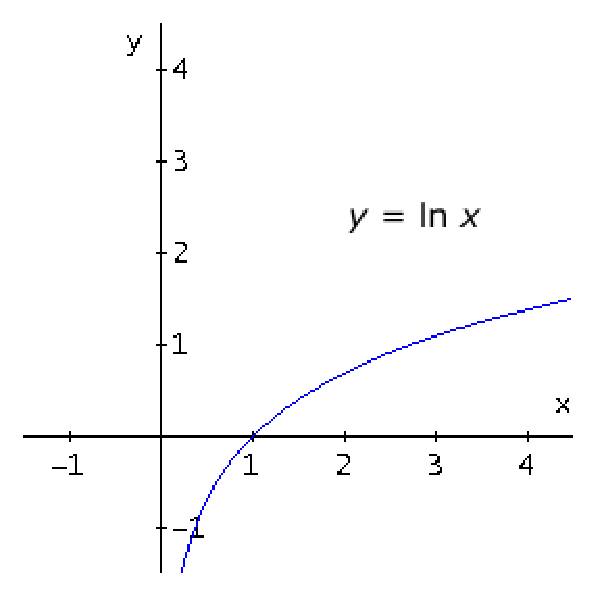
\includegraphics[width=0.50\textwidth]{img/fun053.eps}
\caption{Función Logaritmo Neperiano}
\label{fig:1}
\end{center}
\end{figure}
%------------------------------------------------------------------------------

\end{frame}
%++++++++++++++++++++++++++++++++++++++++++++++++++++++++++++++++++++++++++++++  



%++++++++++++++++++++++++++++++++++++++++++++++++++++++++++++++++++++++++++++++  
\begin{frame}
\section{Conclusiones}
\frametitle{Conclusiones}

  \begin{enumerate}
    \item
     Conclusiones matemáticas:
     Hemos concluido que el Desarrollo de Taylor aplicado a la 
     función logaritmo neperiano de ``x'', fijando dos varibles y variando una, afecta, sobretodo, a la proximidad de la Serie
     de Taylor en f(x)=ln(x) y el valor del Logaritmo Neperiano en ese punto.
      \pause
    \item
     Conclusiones de programación:
     Mediante la realización del trabajo hemos contrastado la información con programas informáticos (Python), por lo cual,
     queda demostrado la eficacia frente a otros métodos.
   \end{enumerate}


\end{frame}

\begin{frame}[fragile]
\tiny{
\frametitle{Algoritmo}
\begin{verbatim}
from sympy import *
import sys
import time
def fac(grado):
  if grado == 0:
    return 1
  else:
    return grado * fac(grado-1)

def taylor(grado, punto, centro):
  Ti=time.time()
  c = Symbol('c')
  funcion = ln(c)
  suma = funcion.evalf(subs={c:centro})
  for i in range(1,grado+1):
    deriv = diff(funcion, c)
    termino = (deriv.evalf(subs={c:centro})/fac(i))*((punto-centro)**i)
    funcion = deriv
    suma += termino
  return suma
  error = funcion- suma
  Tf=time.time() 
  tiempo= Tf-Ti
grado = int(raw_input('Introduzca el grado en el que desea que se aplique el desarrollo de Taylor: '))
punto = float(raw_input('Introduzca el punto en el que desea que se aplique el desarrollo de Taylor: '))
centro = float(raw_input('Introduzca el centro en el que desea que se aplique el desarrollo de Taylor: '))
suma = taylor(grado, punto, centro)
print 'El polinomio de Taylor es: ', suma
Ti=time.time()
Tf=time.time() 
tiempo= Tf-Ti
print 'Tiempo: ', tiempo
\end{verbatim}
}
\end{frame}
%++++++++++++++++++++++++++++++++++++++++++++++++++++++++++++++++++++++++++++++  

%++++++++++++++++++++++++++++++++++++++++++++++++++++++++++++++++++++++++++++++  
\begin{frame}
  \frametitle{Bibliografía}

  \begin{thebibliography}{10}

    \beamertemplatebookbibitems
    \bibitem[Juan de Burgos,2004]{Burgos}  
   Cálculo infinitesimal de una variable 
    (2004) 

    \beamertemplatebookbibitems
    \bibitem[Michael Spivak]{Spivak}  
    Calculus. Cálculo Infinitesimal(2006) 
    
   
    \beamertemplatebookbibitems
    \bibitem{Ln} 
    {\small $http://ordenador.wingwit.com/$}
    
    \beamertemplatebookbibitems
    \bibitem{Ln}
      {\small $http://fr.wikiversity.org/$ }

    \beamertemplatebookbibitems
    \bibitem{Ln} 
    {\small $http://es.scribd.com/$}
    
     \beamertemplatebookbibitems
    \bibitem{Ln} 
    {\small $http://www.slideshare.net/$}
    
     \beamertemplatebookbibitems
    \bibitem{Ln} 
    {\small $http://recursostic.educacion.es/$}
    


  \end{thebibliography}
\end{frame}


%++++++++++++++++++++++++++++++++++++++++++++++++++++++++++++++++++++++++++++++  

\end{document}
